\documentclass[UTF8]{ctexart}    %有中英文时使用

\usepackage{graphicx}  %引用图片包
\graphicspath{{fig/}}
\usepackage{subfigure}
\title{latex学习笔记}
\author{xyn}
\date{\today}

\begin{document}
   \maketitle        %显示前言部分  Ctrl+T快速注释ctrl+u去注释

   \textbf{第一部分}   %加粗

   \newpage
\thispagestyle{empty}
\tableofcontents
\newpage

   \textit{英文斜体yeah}   %斜体

   \underline{下划线}      %标记重点

   \section{第一章节}
   neirong
   \subsection{第一章节子章节}
   子章节内容
   \subsubsection{zizi章节}

   \section{第二部分——图片}

   喀纳斯见图\ref{kanasi}
\begin{figure}[!hb]
   \centering  %图片居中显示        %绝对路径不能有中文
   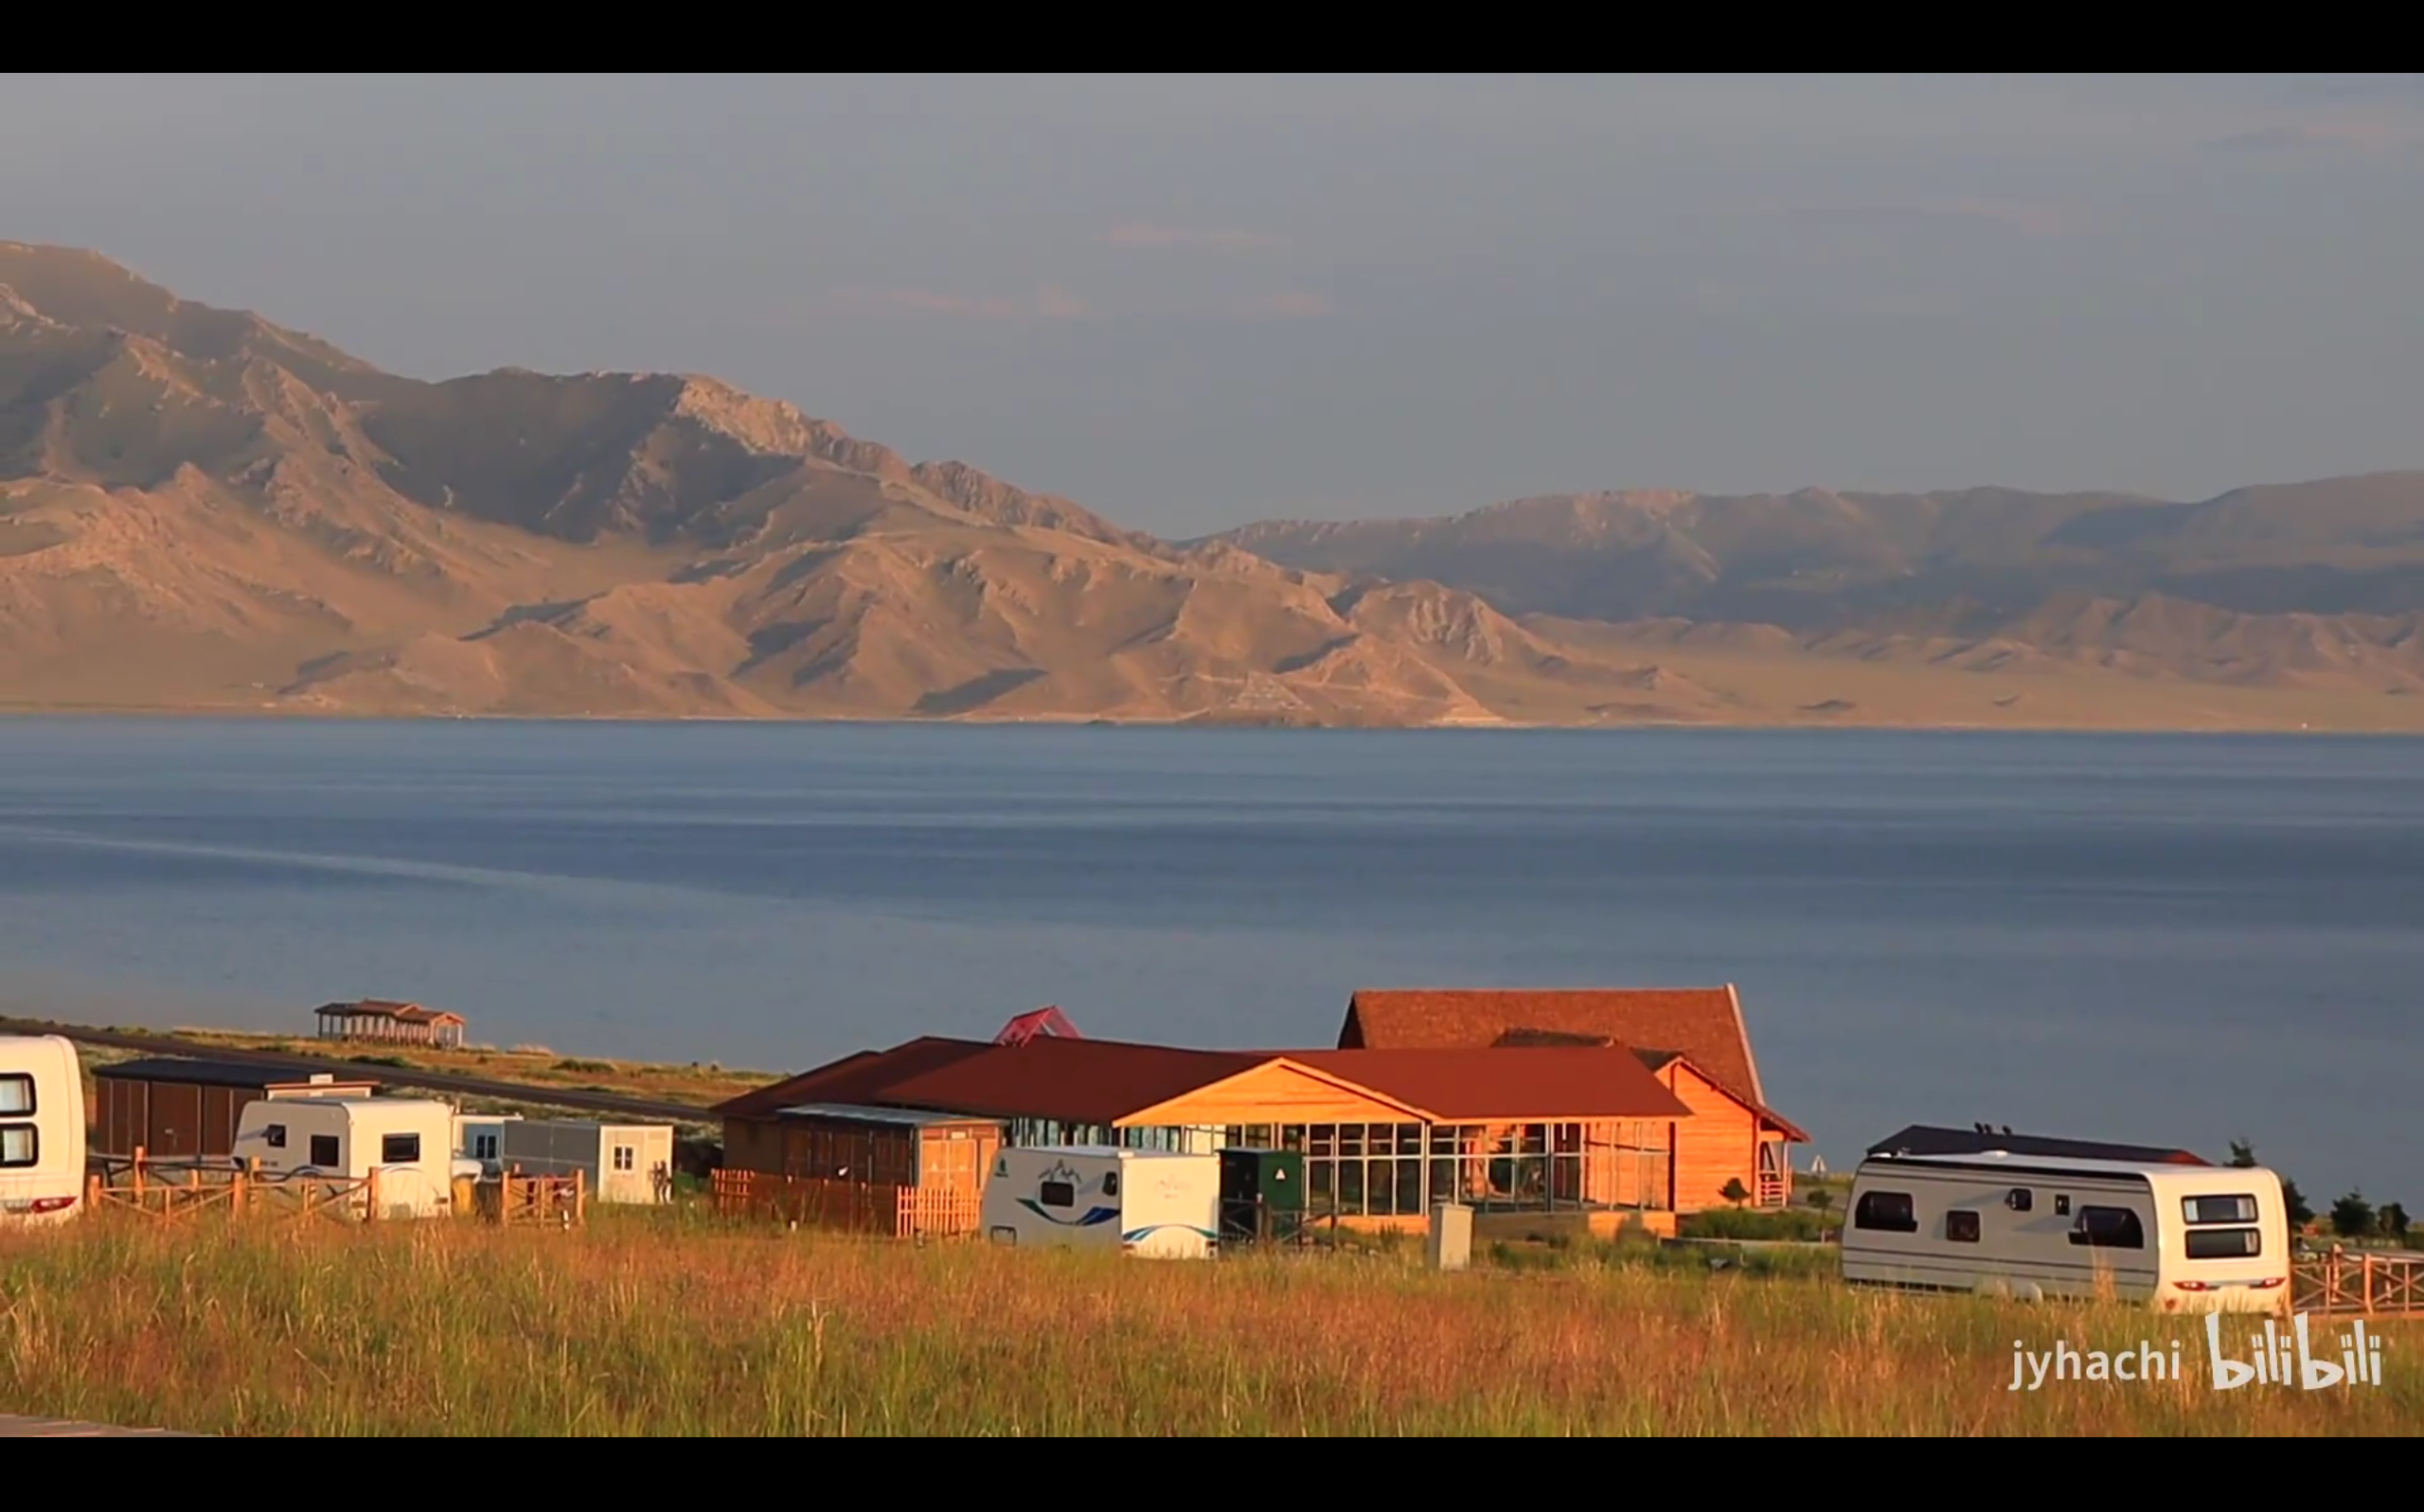
\includegraphics[width=3cm]{jinyue.png}
   \caption{这是美丽喀纳斯} \label{kanasi}
\end{figure}


   jinyuehainan见图\ref{hainan}

\begin{figure}[h]               %并排插图
   \centering
   \subfigure[1]{
       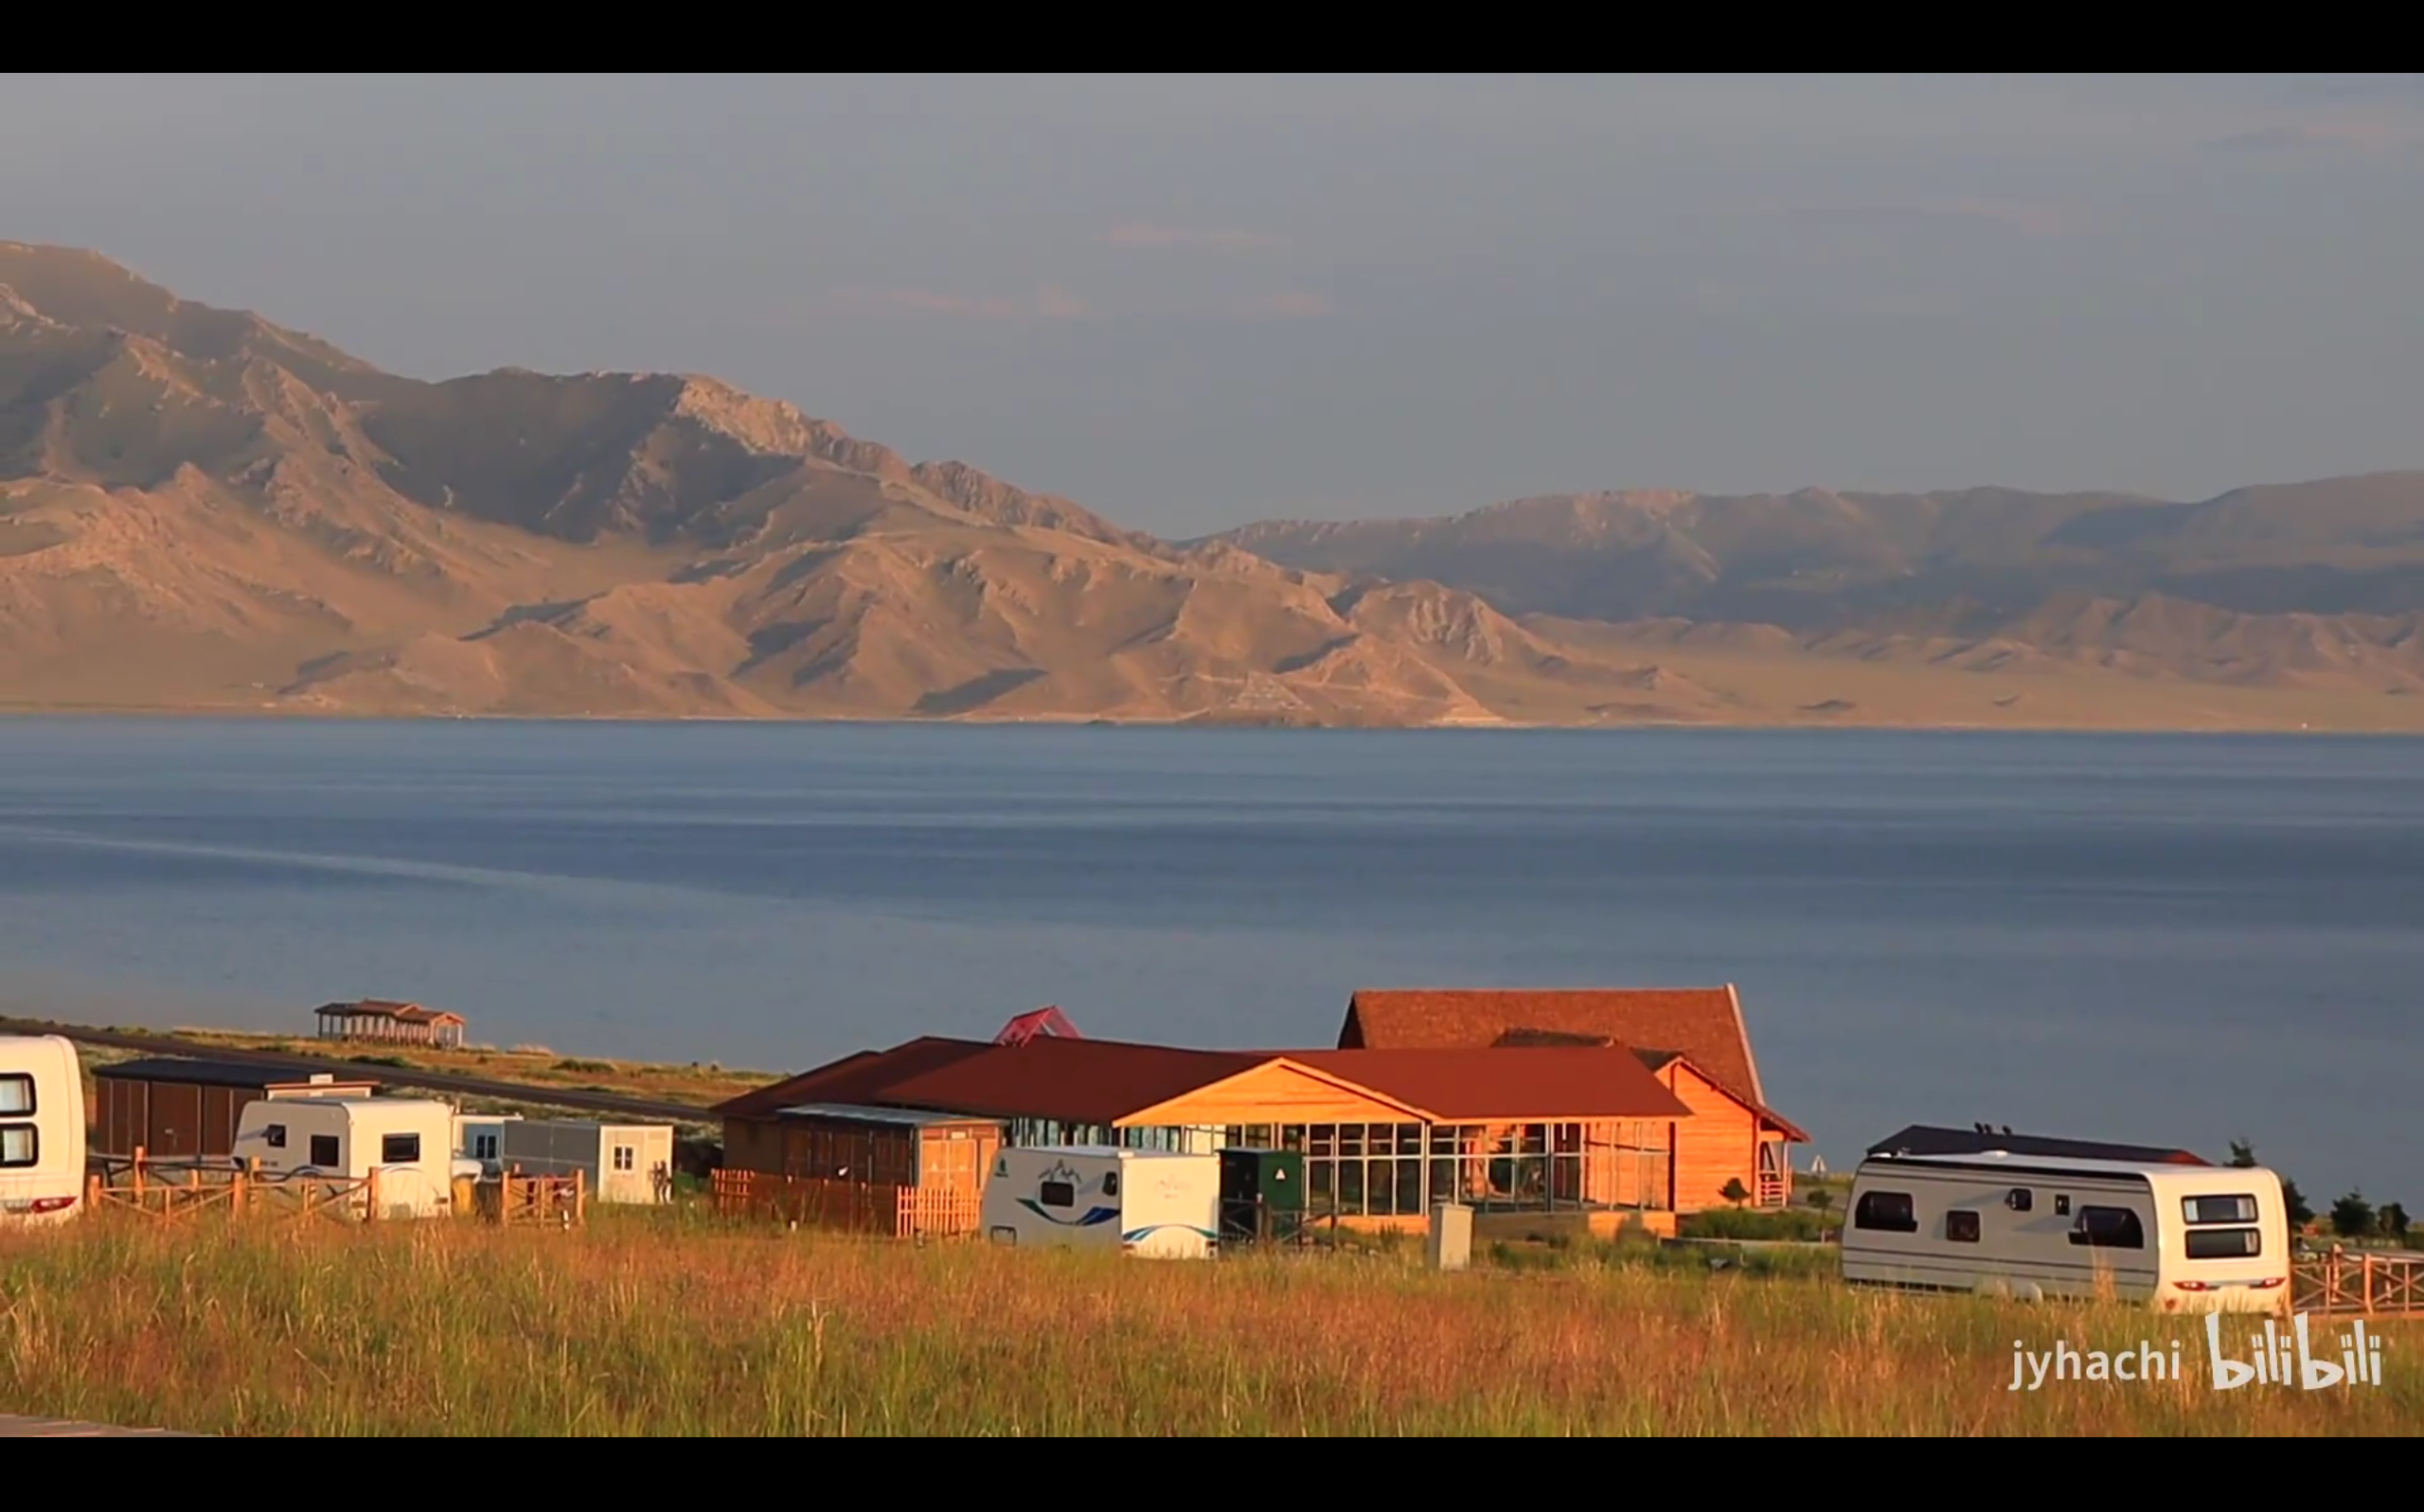
\includegraphics[width=2in]{jinyue.png}}     %使用相对路径
    \hfill
    \centering
   \subfigure[2]{
       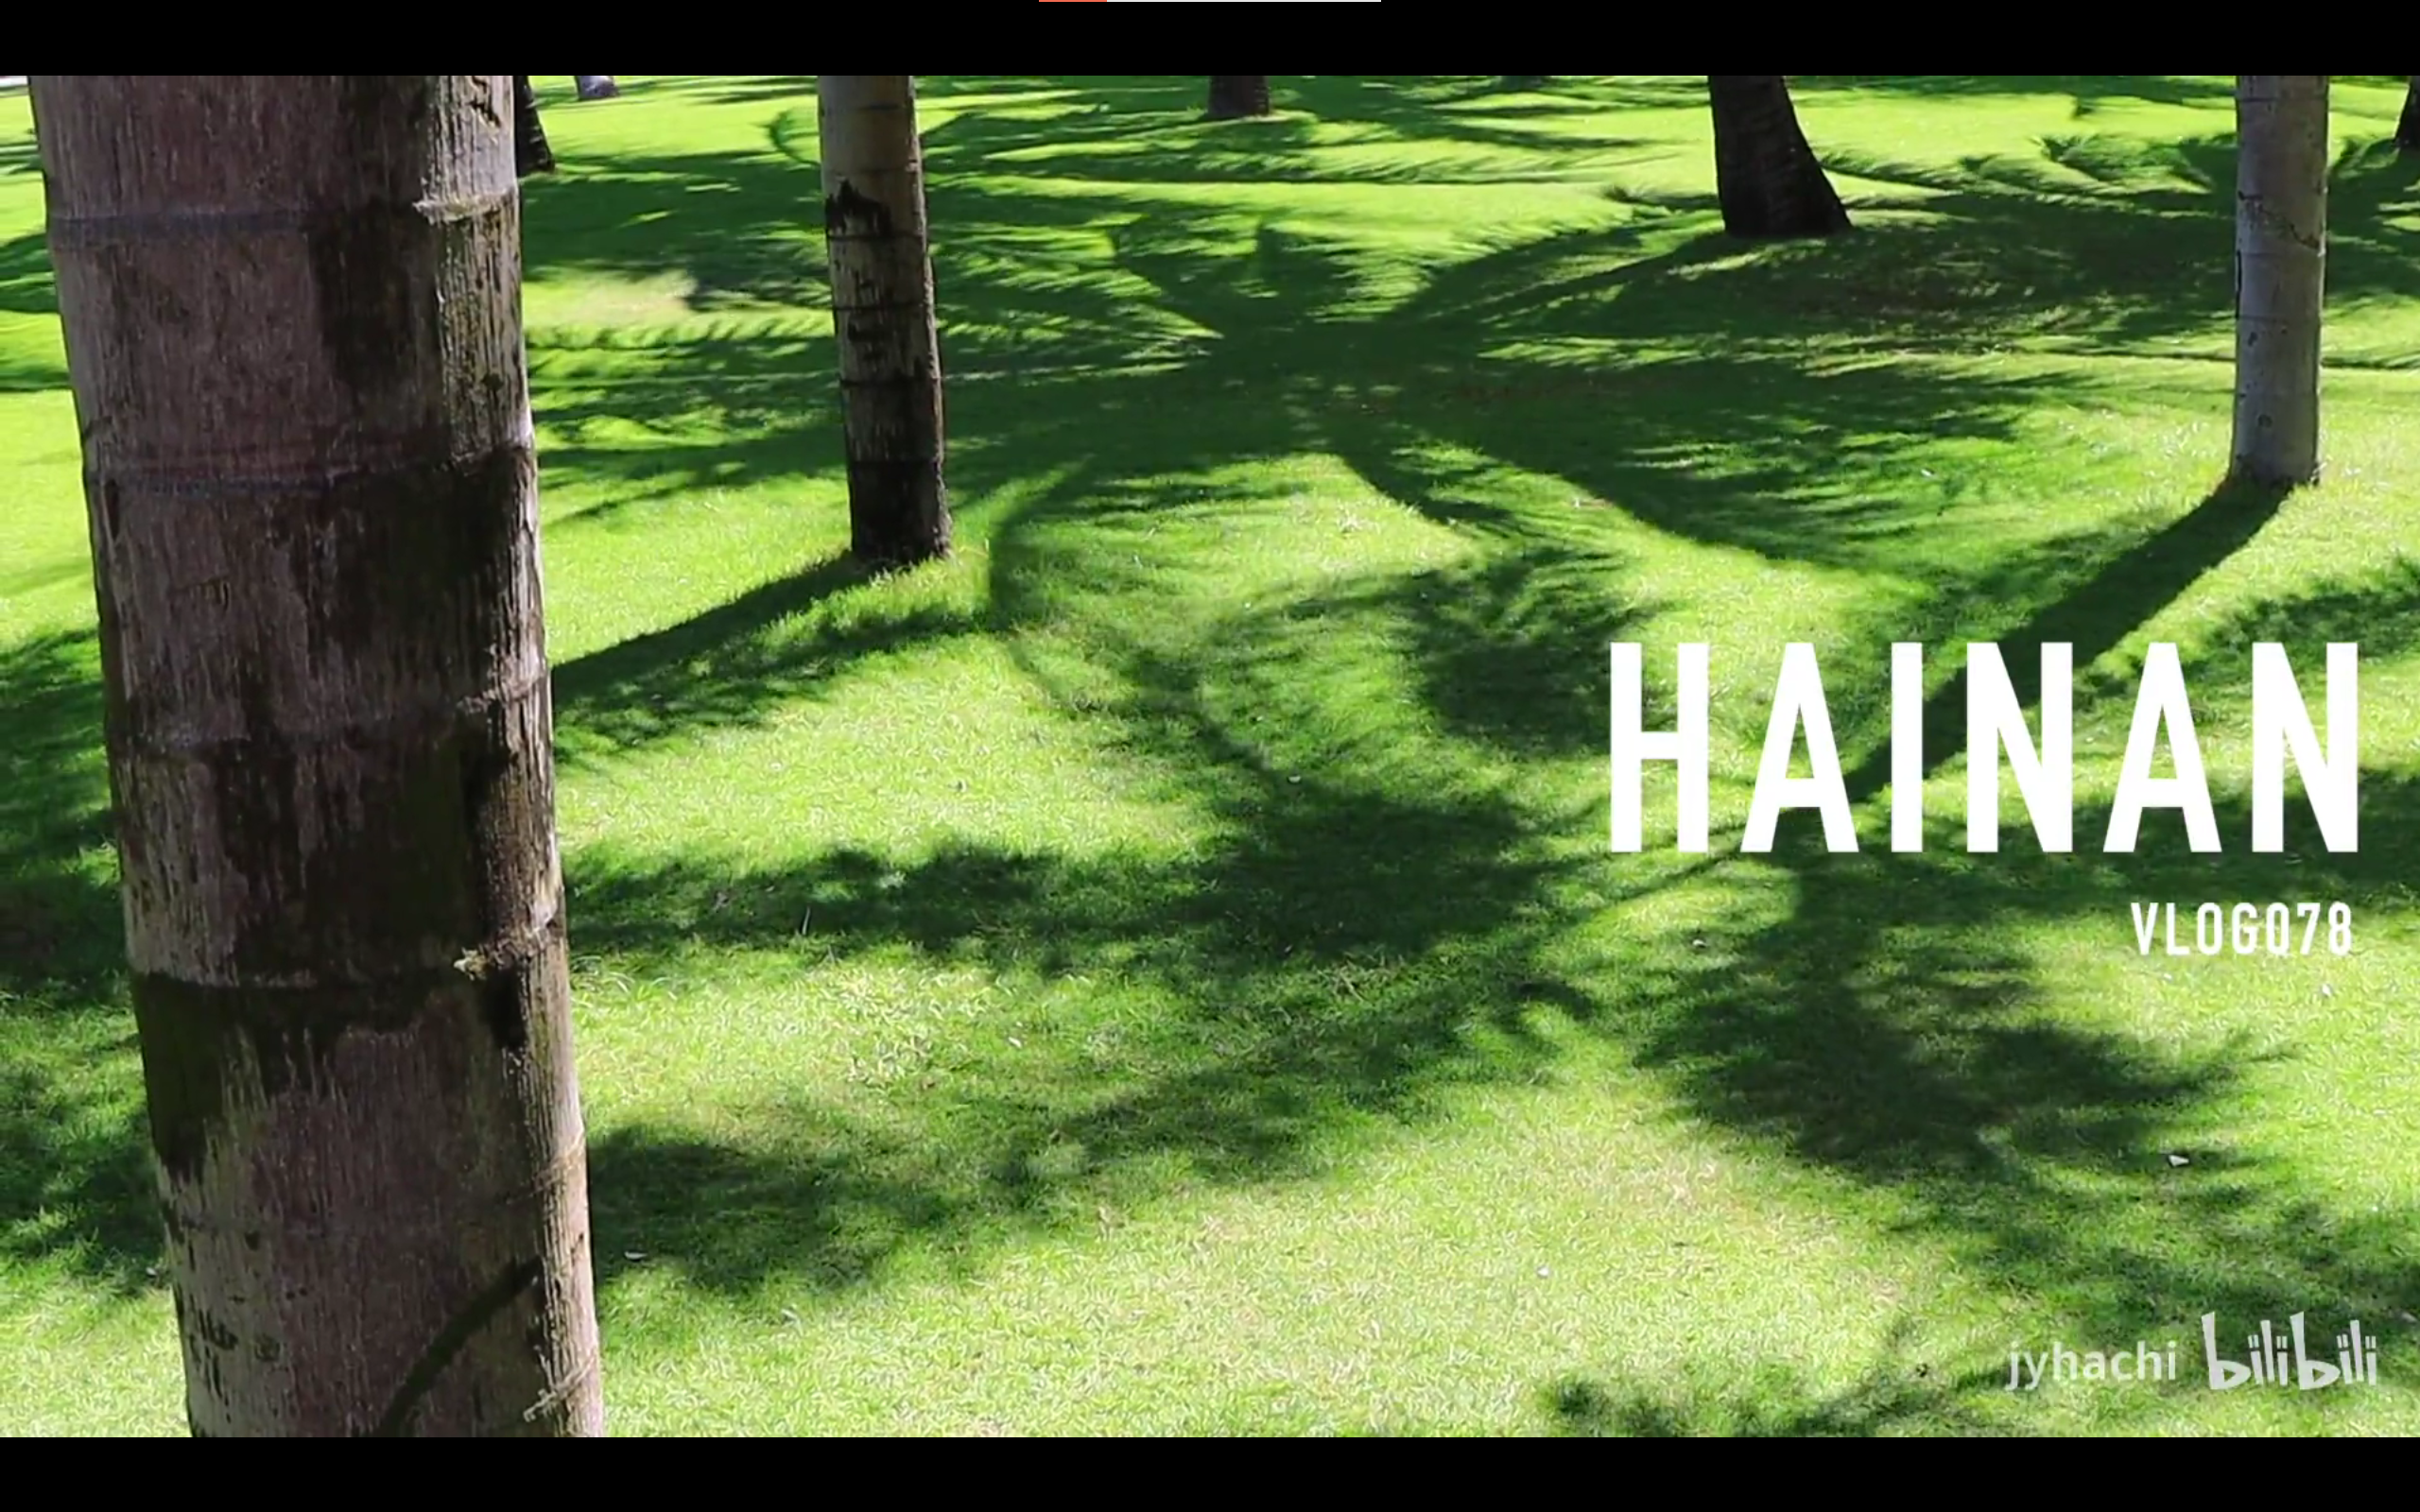
\includegraphics[width=2in]{hainan.png}}
   \caption{hainan}\label{hainan}
\end{figure}



\section{第三部分-列表、表格}
\begin{itemize}    %无序列表
    \item 列1
    \item 列2
    \item 列3
\end{itemize}

\begin{enumerate}    %有序列表  [a.]/[A.]
    \item lie1
    \item lie2
\end{enumerate}

\begin{table}
\begin{tabular}{|l|c|r|p{2cm}|}       %表格环境及左右对齐
\hline                          %横线的添加
左&中&右&r\\
\hline
left&center&right&r\\
\hline
\end{tabular}
\caption{一个标题}
\end{table}


\end{document}

